\setcounter{chapter}{5}

\chapter{定积分及其应用}

\section{定积分的概念与性质}

\subsection{定义}

{\bf 问题:}如何求给定曲线所围平面区域的面积?

\begin{center}
	\resizebox{!}{5.2cm}{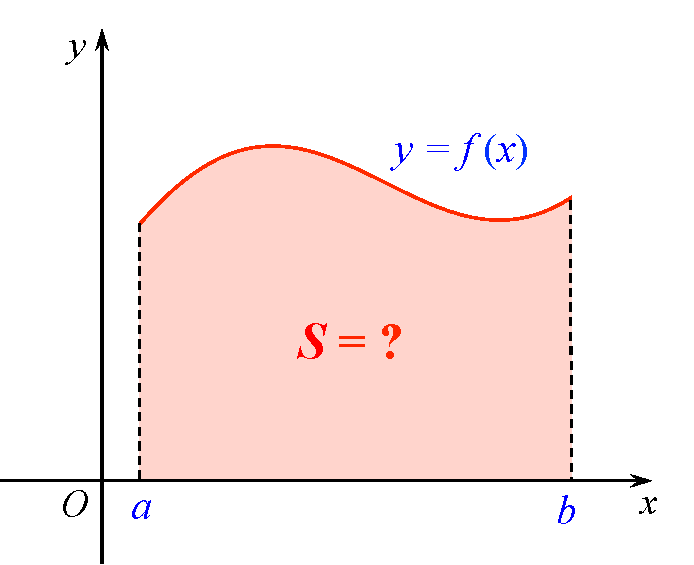
\includegraphics{./images/ch6/integral.pdf}}
	
	$$S=\dint_a^bf(x)\d x$$
\end{center}

{\bf P301-例1:}求由曲线$y=x^2$以及直线$x=0,x=1$和$y=0$所围成的曲边梯形的面积。

\begin{center}
	{\bf “分割取近似,做和求极限”}
\end{center}

{\bf 定义6.1.1:}函数$y=f(x)$在区间$[a,b]$上(Riemann)可积:
$$\dint_a^bf(x)\d x=\lim\limits_{\lambda\to
0}\sum\limits_{k=1}^nf(\xi_k)\Delta x_k$$

{\bf 注:}
\begin{enumerate}[(1)]
  \setlength{\itemindent}{1cm}
  \item 两个“任意”
  \begin{itemize}
    \item 对$[a,b]$的任意分法
    \item 给定分法,$\xi_k$的取法应该是任意的
  \end{itemize}
  \item $\lambda\to 0$用于保证分割得足够“细”
\end{enumerate}

{\bf 定理6.1.1:}
\begin{enumerate}[(1)]
  \setlength{\itemindent}{1cm}
  \item $f(x)$在$[a,b]$上可积,则一定在$[a,b]$上有界 
  \item $f(x)$在$[a,b]$上连续,则一定在$[a,b]$上可积 
\end{enumerate}

{\bf 注:}分段连续(只有有限个第一类间断点)的函数是可积的

{\bf P309-例2:}证明Dirichlet函数在任意区间$[a,b]$上不可积。

{\bf P317-习题7:}将下列求和式表示成定积分 
\begin{enumerate}[(1)]
  \setlength{\itemindent}{1cm}
  \item $\limn\df 1n\left[\sin\df{\pi}{n}+\sin\df{2\pi}{n}+\ldots
  +\sin\df{(n-1)\pi}{n}\right]$ 
  \item $\limn\left(\df{1}{n^2}+\df{2}{n^2}+\ldots+\df{n-1}{n^2}\right)$
\end{enumerate}

{\bf 例:}求$\limn\sum\limits_{k=1}^n\df{k}{n^3}\sqrt{n^2-k^2}$。

{\bf 例:}利用定积分定义证明以下极限:
$$\limn\cos\df x2\cos\df x4\cos\df x8\cdot\cdots\cdot\cos\df x{2^n}
=\df{\sin x}x,$$
并证明Vieta's Formula(韦达公式)
$$\df2\pi=\df{\sqrt2}2\cdot\df{2+\sqrt2}2\cdot\df{\sqrt{2+\sqrt{2+\sqrt2}}}2
\cdot\cdots$$

{[hint]:}
\begin{align}
	&\cos\df x2\cos\df x4\cos\df x8\cdots\cos\df x{2^n}\notag\\
	&=\df12\left(\cos\df34x+\cos\df14x\right)\cos\df x8\cdots\cos\df
	x{2^n}\notag\\
	&=\df1{2^2}\left(\cos\df78x+\cos\df58x+\cos\df38x+\cos\df18x\right)
	\cos\df x{16}\cdots\cos\df x{2^n}\notag\\
	&=\ldots\notag\\
	&=\df1{2^{n-1}}\left(\cos\df{2^n-1}{2^n}x+\cos\df{2^n-3}{2^n}x+
	\ldots+\cos\df3{2^n}x+\cos\df1{2^n}x\right)\notag\\
	&=\dint_0^1\cos(xt)\d t=\df{\sin x}x\notag
\end{align}

{\bf 例:}$G_n=\sqrt[n]{(n+1)(n+2)\cdots(n+n)},(n=1,2,\ldots)$,求
$\limn\df{G_n}n$.

{[hint]:}
$$\ln\df{G_n}n=\limn\df1n\sum\limits_{k=1}^n\ln\left(1+\df kn\right)
=\dint_0^1\ln(1+x)\d x=2\ln2-1$$

\subsection{几何意义}

\begin{center}
	\resizebox{!}{3.12cm}{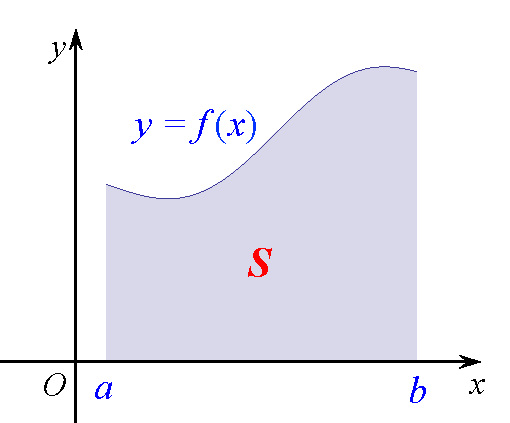
\includegraphics{./images/ch6/IS1.pdf}} 
	\resizebox{!}{3.12cm}{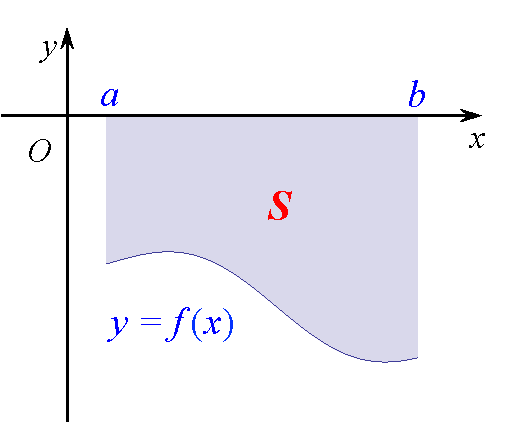
\includegraphics{./images/ch6/IS2.pdf}} 
	\resizebox{!}{3.12cm}{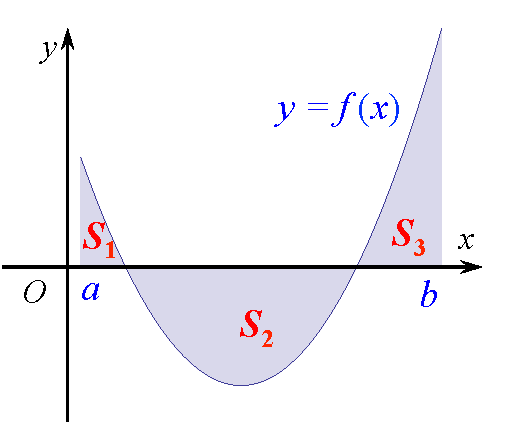
\includegraphics{./images/ch6/IS3.pdf}}
	
	“带符号的面积” 
\end{center}

{\bf 约定:}
\begin{enumerate}[(1)]
  \setlength{\itemindent}{1cm}
  \item $\dint_a^af(x)\d x=0$
  \item $\dint_b^af(x)\d x=-\dint_a^bf(x)\d x$ 
\end{enumerate}

{\bf 例:}$f(x)\in C[0,1]$且严格单调递增,$f(0)=0,f(1)=1$,已知
$\dint_0^1f(x)\d x=\df23$,求$\dint_0^1f^{-1}(y)\d y$

{[hint]:}作图易知
$$\dint_0^1f(x)\d x+\dint_0^1f^{-1}(y)\d y=1$$

\begin{center}
	\resizebox{!}{5cm}{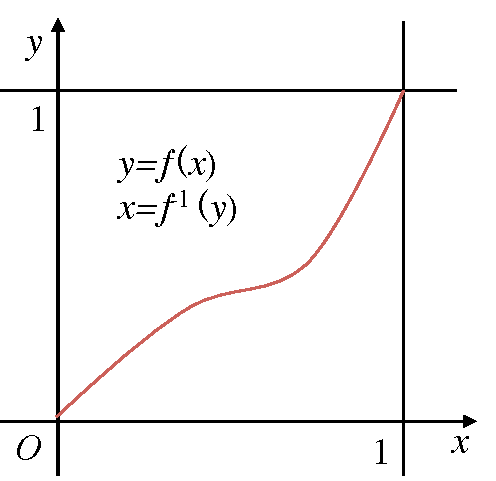
\includegraphics{./images/ch6/iff-1.pdf}}  
\end{center}

{\bf 例:}$a>1$,证明:$\dint_1^a\ln x\d x+\dint_0^{\ln a}e^y\d y=a\ln a$

[hint]:与上题同理。

{\bf 命题:}$f(x)\in C[a,b]$严格单调增加,则
$$\dint_a^bf(x)\d x+\dint_{f(a)}^{f(b)}f^{-1}(y)\d y=bf(b)-af(a)$$
例如:
$$\dint_0^{\pi/2}\sin x\d x+\dint_0^1\arcsin x\d x=\df{\pi}2$$
\begin{center}
	\resizebox{!}{5cm}{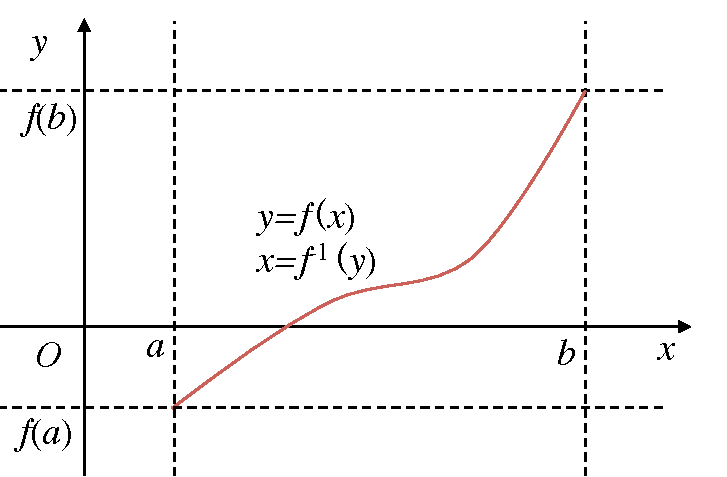
\includegraphics{./images/ch6/iff-1ab.pdf}}  
\end{center}

{\bf 例:}$f(x)\in C[0,+\infty)$且严格单调递增,$f(0)=0,a>0,b>0$,则
成立如下的Young不等式
$$ab\leq\dint_0^af(x)\d x+\dint_0^bf^{-1}(y)\d y$$
\begin{center}
	\resizebox{!}{4cm}{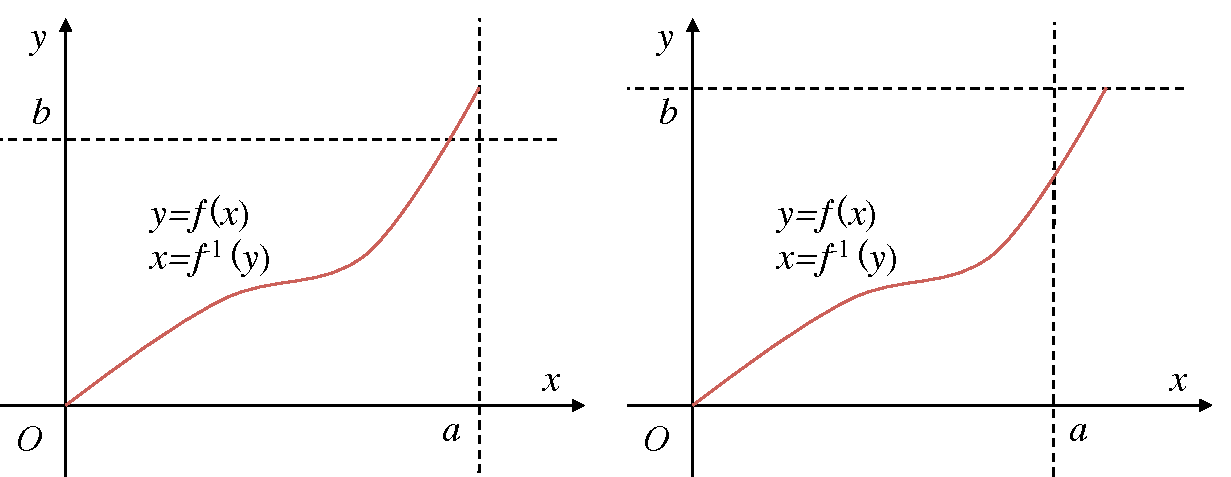
\includegraphics{./images/ch6/iff-ab.pdf}}  
\end{center}
利用该不等式,可以证明Minkowski不等式:设$p>1,q>1,\df1p+\df1q=1$,则
$$ab\leq\df{a^p}p+\df{b^q}q$$
[hint]:令$f(x)=x^{p-1}$,则$x=y^{q-1}$(注意到$\df1{p-1}=q-1$)

{\bf 例:}计算$\dint_0^1\left(\sqrt[3]{1-x^7}-\sqrt[7]{1-x^3}\right)\d x$

[hint]:$y=\sqrt[3]{1-x^7}$和$x=\sqrt[7]{1-y^3}$互为反函数!

\subsection{基本性质}

\begin{enumerate}[(1)]
  \setlength{\itemindent}{1cm}
  \item {\bf 线性性:}
  $$\dint_a^b[\alpha
  f(x)+\beta g(x)]\d x=\alpha\dint_a^bf(x)\d x+\beta\dint_a^bg(x)\d x$$
  \item {\bf 区间可加性:}
  $$\dint_a^bf(x)\d x=\dint_a^cf(x)\d x+\dint_c^bf(x)\d x$$
  \item {\bf 保号性:}
  \begin{itemize}
    \item $f(x)$在$[a,b]$上可积,且$f(x)\geq 0$,则$\dint_a^bf(x)\d x\geq 0$ 
    \item $f(x)$在$[a,b]$上连续,非负且不恒为零,则$$\dint_a^bf(x)\d x> 0$$ 
    \item {\bf 保序性:}设$f(x),g(x)$在$[a,b]$上可积,且$f(x)\leq g(x)$,则
    $$\dint_a^bf(x)\d x\leq \dint_a^bg(x)\d x$$
    \item {\bf 绝对值不等式:}$f(x)$在$[a,b]$上可积,则
    $$\dint_a^bf(x)\d x\leq\dint_a^b|f(x)|\d x$$ 
    \item {\bf 积分估值:}$f(x)$在$[a,b]$上可积,且$m\leq f(x)\leq M$,则
    $$m(b-a)\leq\dint_a^bf(x)\d x\leq M(b-a)$$
  \end{itemize}
\end{enumerate}

\subsection{定积分中值定理}

{\bf 定理6.1.2:}若函数$f(x)$在区间$[a,b]$上连续,则在$[a,b]$上至少存在一点$\xi$,使得
$$\dint_a^bf(x)\d x=f(\xi)(b-a)$$

{\bf 注:}定积分中值定理与微分中值定理有何联系?

{\bf 例:}计算如下极限
$$\limx{+\infty}\sqrt[3]x\dint_x^{x+1}\df{\sin t}{t+\cos t}\d t$$

\section{微积分基本公式与定积分的计算}

\subsection{微积分基本公式}

{\it 在Newton和Leibniz之前,微分和积分的许多个别结果已经得到,但只有当
他们发现了这个公式之后,微积分才统计成了一个整体!}

{\bf P319-例6.2.1:}设函数$f(x)$在区间$[a,b]$上可积,$F(x)$是
$f(x)$在$[a,b]$上的一个原函数,则
$$\dint_a^bf(x)\d x=F(b)-F(a).$$

{\bf P320-例1:}计算定积分
\begin{enumerate}[(1)]
  \setlength{\itemindent}{1cm}
  \item $\dint_{0}^{1}x^2 \d x$
  \item $\dint_{-1}^{\sqrt 3}\df 1{1+x^2}\d x$
  \item $\dint_{-1}^{-2}\df 1x\d x$
\end{enumerate}

{\bf 例:}如下的计算过程有什么错误?
$$\dint_0^{3\pi/4}\df{\sin x}{1+\cos^2x}\d x
=\left.\arctan(\sec x)\right|_0^{3\pi/4}=-\arctan\sqrt2-\df{\pi}4$$
正确的方法
$$\dint_0^{3\pi/4}\df{\sin x}{1+\cos^2x}\d x
=-\dint_0^{3\pi/4}\df{\d\cos x}{1+\cos^2x}=\arctan\df{\sqrt2}2
+\df{\pi}4$$

{\bf 注:}定积分计算中使用换元法时,必须同时将积分上下限更改为对应的值,且必须保证
变换后的变量是连续变化的!!

{\bf 例:}如下的计算过程有什么错误?
$$\dint_0^{\pi}\df{\d x}{2+\cos2x}=\df1{\sqrt3}\arctan
\left(\df{\tan x}{\sqrt3}\right)_0^{\pi}=0$$
错误:原函数在$x=\pi/2$处有间断点!正确的过程
\begin{align}
	\dint_0^{\pi}\df{\d x}{2+\cos2x}&=\dint_0^{\pi}\df{\d x}
	{3-2\sin^2x}=\dint_0^{\pi}\df{\cot^2x\d x}{3\csc^2x-2}\notag\\
	&=-\dint_0^{\pi}\df{\d\cot x}{3\cot^2x+1}=\df{\pi}{\sqrt3}\notag
\end{align}

{\bf 注:}
\begin{itemize}
  \setlength{\itemindent}{1cm}
  \item 可积函数未必有原函数,例如,有第一类间断点的函数
  \item 有原函数的函数未必可积,例如
  $$f(x)=x^2\sin\df1x,(x\ne0), 0$$
\end{itemize}

{\bf 例:}设$f(x)$满足方程
$$f(x)=3x-\sqrt{1-x^2}\dint_0^1f\,^2(x)\d x,$$
求$f(x)$。

{\bf 例:}求$F(x)=\dint_0^x[\,t\,]\d t,\;(x>0)$的表达式,其中$[\,x\,]$为下取整函数。

\subsection{变限积分}

{\bf 定理6.2.2:}若$f(x)$在$[a,b]$上可积,则{\it 变上限积分}
$$\Phi(x)=\dint_a^xf(t)\d t$$
在$[a,b]$上连续。

{\bf 定理6.2.3:}若$f(x)$在$[a,b]$上连续,则$\Phi(x)=\dint_a^xf(t)\d t$在$[a,b]$可导,且
$$\Phi'(x)=f(x)$$

{\bf 注:}若$f(x)$连续,则变上限积分$\Phi(x)=\dint_a^xf(t)\d t$是$f(x)$的一个原函数

{\bf 思考:}为什么$\Phi(x)$是$f(x)$的“一个”原函数?

$${\left[\dint_{\varphi(x)}^{\psi(x)}f(t)\d t\right]'_x
	=f[\psi(x)]\psi'(x)-f[\varphi(x)]\varphi'(x)}$$

{\bf P325-例6:}求下列函数的导函数
\begin{enumerate}[(1)]
  \setlength{\itemindent}{1cm}
  \item $y=\dint_0^{x}e^{-t^2}\d t$
  \item $y=\dint_0^{x^2}\sqrt{1+t^4}\d t$
  \item $y=\dint_{-x}^{\sqrt x}\sin t^2\d t$
\end{enumerate}

{\bf P329-例13:}设$f(x)$在$[0,+\infty)$内连续,且$f(x)>0$,证明:
$$F(x)=\df{\dint_0^xtf(t)\d t}{\dint_0^xf(t)\d t}$$
在$(0,+\infty)$内单调递增。

{\bf P330-例14:}设$f(x)$在$[0,+\infty)$上可导,$f(0)=0$,且存在反函数$g(x)$,已知
$$\dint_0^{f(x)}g(t)\d t=(x-1)e^x+x^2+1,$$
求$f(x)$。

{\bf 例:}设$\limx{0}\df{1}{bx-\sin
x}\dint_0^x\df{t^2}{\sqrt{a+t}}\d t=1$,求$a,b$。

{\bf 例:}设$\phi(x)=\dint_a^x(x+t)\varphi(t)\d t$,其中$\varphi(x)$可导,求
$\phi''(x)$。

{\bf 思考:}若$\phi(x)=\dint_a^x(x+t)\varphi(x+t)\d t$,结果如何?

{\bf 例:}$x>0$时,$\cos x\leq 1$,该式从$0$到$x$积分可得
$$\sin x\leq x$$
进而
$$1-\cos x<\df{x^2}2$$
$$\sin x>x-\df{x^3}6$$
$$\ldots$$
最终
$$\left|\sin x-\sum\limits_{k=0}^n(-1)^k\df{x^{2k+1}}{(2k+1)!}\right|
\leq\df{|x|^{2n+3}}{(2n+3)!}$$
$$\left|\cos x-\sum\limits_{k=0}^n(-1)^k\df{x^{2k}}{(2k)!}\right|
\leq\df{|x|^{2n+2}}{(2n+2)!}$$

\begin{shaded}
	{\bf 积分中值定理的证明及其应用}
	
	利用变限积分的性质和Cauchy中值定理,可以证明定积分中值定理。

	{\bf 例:}设$f(x)$在$[a,b]$上连续,且$g(x)$在$[a,b]$上可积且不变号,证明:存在
	$\xi\in(a,b)$,使得
	$$\dint_a^bf(x)g(x)\d x=f(\xi)\dint_a^bg(x)\d x$$
	
	{\bf [hint]:}let $F(t)=\dint_a^tf(x)\d x,\;G(t)=\dint_a^tg(x)\d x$,则
	由Cauchy中值定理
	$$\df{F(b)-F(a)}{G(b)-G(a)}=\df{F'(\xi)}{G'(\xi)}=f(\xi)$$
	
	{\bf 例:}计算极限$\limn f(n)\sin\df 1n$,其中
	  $$f(x)=\dint_x^{x^2}\left(1+\df 1{2t}\right)^t\sin\df{1}{\sqrt t}\d t$$
	
	{\bf [hint]:}
	\begin{align}
		\limn f(n)\sin\df 1n&=\limn\df1n\dint_n^{n^2}\left(1+\df
		1{2t}\right)^t\sin\df{1}{\sqrt t}\d t\notag\\
		&=\limn\df1n\left(1+\df1{2\xi}\right)^{\xi}\dint_n^{n^2}
		\sin\df1{\sqrt t}\d t\quad(\xi\in(n,n^2))\notag\\
		&=2e^{1/2}\limn\df1n\dint_{\sqrt n}^n2x\sin\df1x\d x\notag\\
		&=2e^{1/2}\limn\eta\sin\df1{\eta}\df{n-\sqrt n}n\quad(\eta\in(\sqrt
		n,n))\notag\\
		&=2e^{1/2}\notag
	\end{align}
	
	{\bf 例:}设$f(x)$在$[0,2\pi]$上连续,证明:
	$$\limn\dint_0^{2\pi}f(x)|\sin nx|\d x=\df 2{\pi}\dint_0^{2\pi}f(x)\d x$$
	
	{\bf [hint]:}
	\begin{align}
	\dint_0^{2\pi}f(x)|\sin nx|\d x
	&=\sum\limits_{k=1}^n\dint_{2(k-1)\pi/n}^{2k\pi/n}f(x)|\sin nx|\d x\notag\\
	&=\sum\limits_{k=1}^nf(\xi_k)\dint_{2(k-1)\pi/n}^{2k\pi/n}|\sin nx|\d x\notag
	\end{align}
	and
	$$\dint_{2(k-1)\pi/n}^{2k\pi/n}|\sin nx|\d x=\df4n$$
	hence
	$$\dint_0^{2\pi}f(x)|\sin nx|\d x=\df4n\sum\limits_{k=1}^nf(\xi_k)
	=\df2{\pi}\left(\sum\limits_{k=1}^nf(\xi_k)\df{2\pi}n\right)$$
\end{shaded}

\subsection{定积分的计算}

{\bf 定理6.3.3}(换元法)
设$f(x)$在$[a,b]$上连续,函数$x=\varphi(t)$满足:
\begin{enumerate}[(1)]
  \setlength{\itemindent}{1cm}
  \item $\varphi(\alpha)=a,\;\varphi(\beta)=b$;
  \item $\varphi(t)$在$[\alpha,\beta]$上连续可导,且$\varphi(t)\in[a,b]$,则
\end{enumerate}
$${\dint_a^bf(x)\d
x=\dint_{\alpha}^{\beta}f[\varphi(t)]\varphi'(t)\d t}$$

{\bf 定理6.3.4}(分部积分法)
$${\dint_a^bu(x)\d v(x)=u(x)v(x)|_a^b-\dint_a^bv(x)\d u(x)}$$

{\bf 例:}计算积分
\begin{enumerate}[(1)]
  \setlength{\itemindent}{1cm}
  \item  $\dint_9^4\df 1{\sqrt x}\d x$ 
  \item $\dint_0^1\sqrt{(1-x^2)^3}\d x$ 
  \item $\dint_0^{\ln 2}\sqrt{1-e^{-2x}}\d x$
  \item $\dint_0^{2\pi}\sqrt{1+\cos\theta}\d\theta$ 
  \item $\dint_0^{\pi}(x\sin x)^2\d x$ 
  \item $\dint_0^{n\pi}x|\sin x|\d x$ 
  \item $\dint_0^1\df{\ln(1+x)}{1+x^2}\d x$
\end{enumerate}

{\bf 例:}设$f(x)=\dint_1^x\df{\ln t}{1+t}\d t$,求$f(x)+f
\left(\df1x\right)$。

{\bf 例:}设$f(\pi)=2$,$\dint_0^{\pi}[f(x)+f''(x)]\sin x\d x=5$,求$f(0)$。

\begin{shaded}
	{\bf 用定积分的性质证明不等式}
	
	{\bf P317-习题10}(Schwarz积分不等式)设$f(x),g(x)$均在$[a,b]$上连续,证明:
	$$\left[\dint_a^bf(x)g(x)\d x\right]^2
	\leq\dint_a^bf\,^2(x)\d x\dint_a^bg^2(x)\d x$$
	
	[hint]:不妨设$\dint_a^bf^2(x)\d x>0$,对任意$t\in\mathbb{R}$
	$$\dint_a^b(tf-g)^2\d x=t^2\dint_a^bf^2\d x-2t\dint_a^bfg\d x
	+\dint_a^bg^2\d x\geq 0$$
	故必有
	$$\Delta=\left(\dint_a^bfg\d x\right)^2-\dint_a^bf^2\d x\dint_a^b
	g^2\d x<0$$
	若$\dint_a^bf^2\d x=\dint_a^b g^2\d x=0$,则
	$$\left|\dint_a^bfg\d x\right|\leq\dint_a^b|fg|\d x
	\leq\dint_a^b\df12(f^2+g^2)\d x=0$$
	
	{\bf 注:}利用该结论可证明Cauchy不等式
	$$\left(\sum\limits_{i=1}^na_ib_i\right)\leq
	\sum\limits_{i=1}^na_i^2\sum\limits_{i=1}^nb_i^2$$
	
	{\bf 例:}$f(x)\in C[a,b]$,且$f(x)>0$,则
	$$\dint_a^bf(x)\d x=\dint_a^b\df1{f(x)}\d x\geq(b-a)^2$$
	
	{\bf 例:}设$f(x)$在$[a,b]$上连续可微,$f(a)=0$,证明:
	$$\dint_a^b[f(x)]^2\d x\leq\df{(b-a)^2}{2}\dint_a^b[f\,'(x)]^2\d x$$
\end{shaded}

{\bf 例:}证明:
$$\dint_1^af\left(x^2+\df{a^2}{x^2}\right)\df{\d x}{x}
=\dint_1^af\left(x+\df{a^2}{x}\right)\df{\d x}{x}$$

{\bf [hint]:}let $y=\df ax$, then
$$\mbox{left}=\df12\dint_1^{a^2}f\left(y+\df{a^2}y\right)\df{\d y}y$$
let $y=\df{a^2}x$, then
$$\dint_a^{a^2}f\left(x+\df{a^2}x\right)\df{\d x}x
=\dint_1^af\left(y+\df{a^2}y\right)\df{\d y}y$$
that is it.

\subsection{定积分的一些特殊计算方法}

\subsubsection{对称区间上的定积分}

{\bf 命题:}$f(x)$连续,则
$$\dint_0^af(x)\d x=\dint_0^af(a-x)\d x$$
利用该结论可以较为简便地计算如下的积分:
\begin{enumerate}[(1)]
  \setlength{\itemindent}{1cm}
  \item $\dint_0^a\df{f(x)\d x}{f(x)+f(a-x)}$
  \item $\dint_0^3\df{\sqrt x\d x}{\sqrt x+\sqrt{3-x}}$
  \item $\dint_0^1\df{x\d x}{e^x+e^{1-x}}$
  \item $\dint_0^{\pi/2}\df{\sin x\d x}{\sin x+\cos x}$
  \ps{在$[0,\pi/2]$上的积分中$\cos x$和$\sin x$可以相互替换}
  \item $\dint_0^{\pi/2}\df{\sin^nx\d x}{\sin^nx+\cos^nx}$
  \item $\dint_0^{\pi}\df{\cos x}{\sqrt{a^2\sin^2x+b^2\cos^2x}}\d
  x\;\;(a^2+b^2\ne 0)$
  \item $\dint_0^{\pi}\df{a^n\sin^2x+b^n\cos^2x}
  {a^{2n}\sin^2x+b^{2n}\cos^2x}\d x$
  \item $\dint_0^{\pi}\df{x\d x}{1+\cos^2x}$
  \item $\dint_0^{\pi}\df{x\sin x\d x}{1+\cos^2x}=\df{\pi^2}4$
  \item $\dint_0^1\df{\ln(1+x)\d x}{1+x^2}=\dint_0^{\pi/4}\ln(1+\tan x)\d x$
  
  [hint]:
  $$\ln\left[1+\tan\left(\df{\pi}4-t\right)\right]=\ln2-\ln(1+\tan t)$$
  故$\ln(1+\tan t)-\df{\ln2}2$是以$\df{\pi}8$为中心的奇函数。于是$I=\df{\pi}8\ln2$
\end{enumerate}

{\bf 例:}利用对称性计算下列各题:
\begin{enumerate}[(1)]
  \setlength{\itemindent}{1cm}
  \item $\dint_{-\pi/2}^{\pi/2}\df{\sin^2x}{1+e^{-x}}\d x$
  \item $\dint_{-1}^1\df{x+\cos x}{1+\sin^2x}\d x$
  \item $\dint_{0}^{\pi}|\cos x|\sqrt{1+\sin^2x}\d x$
  \item $\dint_{-2}^2x\ln(1+e^x)\d x$
\end{enumerate}

\subsubsection{周期函数的定积分}

$$\dint_a^{a+T}f(x)\d x=\dint_0^{T}f(x)\d x$$

\subsubsection{用几何意义计算定积分}

{\bf 例:}$2\dint_{-1}^1\sqrt{1-x^2}\d x=
\dint_{-1}^1\df{\d x}{\sqrt{1-x^2}}$

[hint]:左边是面积,右边为周长

\begin{shaded}
	{\bf 勾股定理的推广}
	
	{\bf 命题:}若$a^2+b^2=c^2$,$f(x)$非负连续,
	$$g(x)=\df acf\left(\df cax\right),\quad 
	h(x)=\df bcf\left(\df cbx\right)$$
	则
	$$\dint_0^xf(x)\d x=\dint_0^xg(x)\d x+\dint_0^xh(x)\d x$$
	\begin{center}
		\resizebox{!}{5cm}{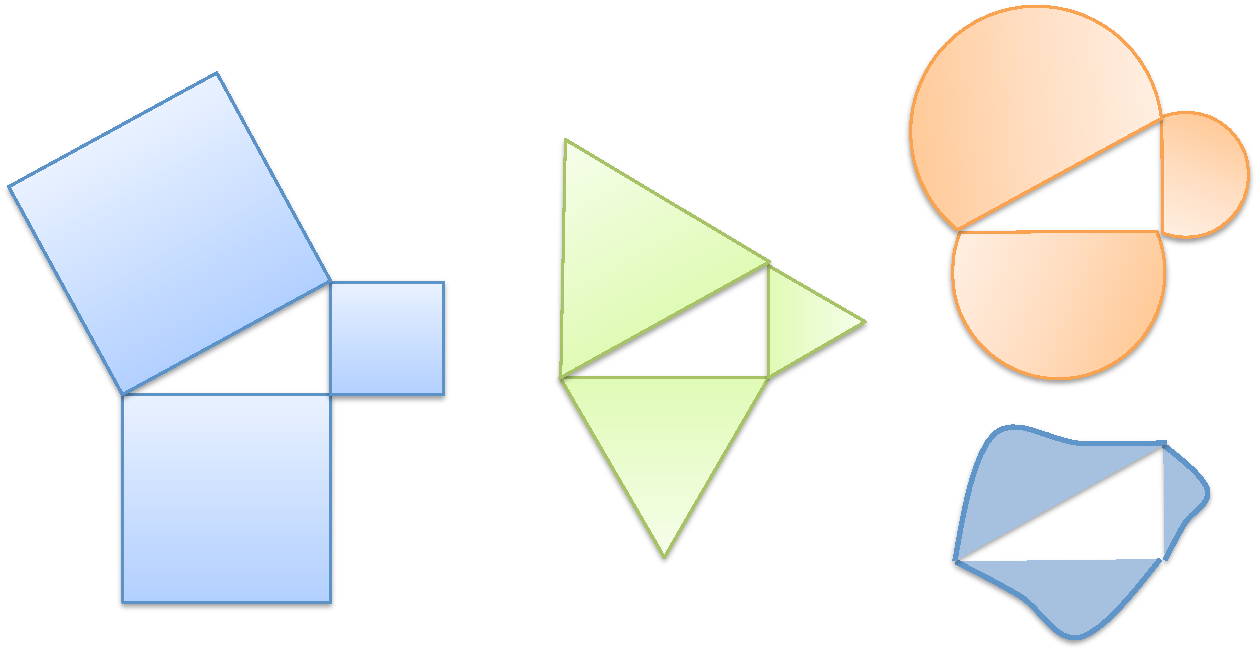
\includegraphics{./images/ch6/ggNew.pdf}}  
	\end{center}
\end{shaded}

% \subsubsection{正弦、余弦的转换}
% 
% $$\dint_0^{\pi/2}f(\sin
% 	  x)\d x=\dint_0^{\pi/2}f(\cos x)\d x$$
	  
{\bf 例:}
$$I=\dint_0^{\pi/2}\df{\cos x}{\sin x+\cos x}\d x$$

\section{定积分的应用}

{\bf 定积分的构造思路──微元法:}

\begin{enumerate}
  \item {\bf 分割:}沿$x$轴方向分割曲边梯形 
  \item {\bf 取近似:}用小矩形的面积$\Delta S$近似小曲边梯形面积 
  \item {\bf 做和:}求所有小矩形的面积总和$\sum \Delta S$ 
  \item {\bf 求极限:}$\sum \Delta S\to S$
\end{enumerate}

\begin{center}
	\resizebox{!}{5.5cm}{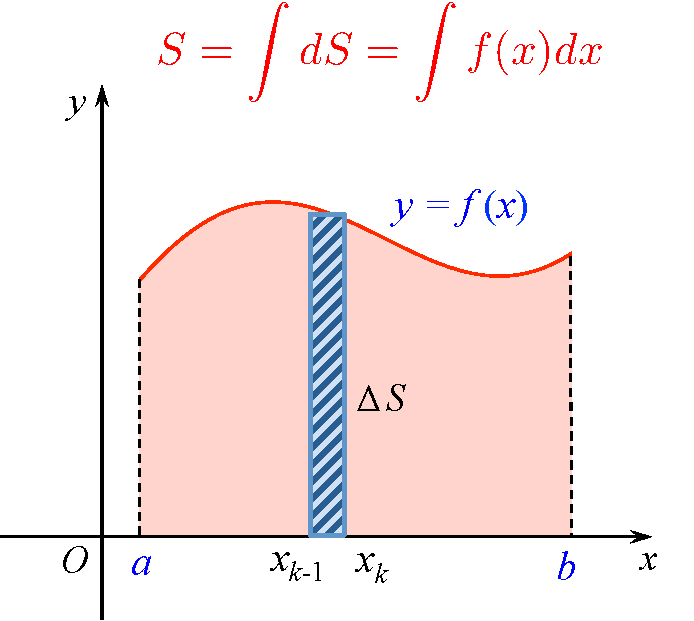
\includegraphics{./images/ch6/sumSSS.pdf}}
\end{center}

\subsection{用定积分求解几何问题}

\subsubsection{面积}

{\bf 例:}计算两条抛物线$y^2=x$和$y=x^2$所围图形的面积。

{\bf 例:}计算两条抛物线$y^2=2x$与直线$y=x-4$所围图形的面积。

{\bf 例:}推导圆和扇形的面积公式。

\subsubsection{极坐标下的面积}

{\bf 例:}计算Archimedes螺线$\rho=a\theta\;(a>0)$
相应于$\theta$从$0$变到$2\pi$的一段弧与极轴所围的图形面积。

\begin{center}
	\resizebox{!}{4cm}{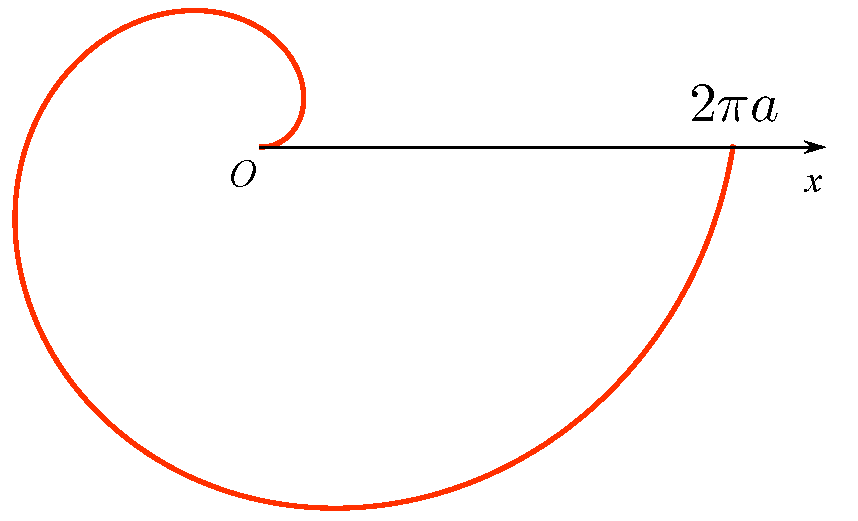
\includegraphics{./images/ch6/Achimedes.pdf}}
\end{center}

{\bf 例}(老羊三问题)
\begin{enumerate}[(1)]
  \setlength{\itemindent}{1cm}
  \item 半径为$a$的圆形水池,一只老羊被长为$ka(0<k\leq2)$的绳子拴在水池边缘,求
  老羊能吃到的草地面积
  \item 如果将水池围起来,老羊吃草时,绳子因为被绕在栅栏上而不能穿过水池,再求面积
  \item 在草场中央围一个半径为$a$的区域,要使内外的老羊吃到的草面积一样,$k$如何取
\end{enumerate}

[hint]:(1)
$$A=\pi k^2a^2-2\dint_{\arccos\frac k2}^{\pi}\df12(2a\cos\varphi)^2
\d\varphi$$
$$A=a^2\left[(k^2-1)\pi+(2-k^2)\arccos\df k2+\df k2
\sqrt{4-k^2}\right]$$
(2)
$$A=\df{\pi k^2a^2}2+2\dint_0^k\df12(ka-a\varphi)^2\d\varphi=k^2a^2
\left(\df{\pi}2+\df k3\right)$$
以上的$\varphi$为小园的圆心角
(3)$k=1.26$

\subsubsection{平面曲线的弧长}

{\bf 例:}求以下曲线的弧长 
\begin{enumerate}[(1)]
  \setlength{\itemindent}{1cm}
  \item $y=\df 23x^{3/2}\;(a\leq x\leq b)$ 
  \item $x=a(t-\sin t),y=a(1-\cos t)\;(0\leq t\leq 2\pi)$ 
  \item $\rho=a\theta\;(a>0,\;0\leq t\leq 2\pi)$
\end{enumerate}

\subsubsection{旋转体的体积}

圆盘法:曲线$y=f(x)\;(x\in[a,b])$与$x=a,x=b,y=0$所围区域绕$x$轴旋转一周:
$$V=\dint_a^b\pi[f(x)]^2\d x$$

{\bf 例:}求椭圆$\df{x^a}{a^2}+\df{y^2}{b^2}=1$绕$x$轴旋转一周所得立体的体积。

圆柱壳法:$y=f(x)\;(x\in[a,b])$与$x=a,x=b,y=0$所围区域绕$y$轴旋转一周
$$V=2\pi\dint_a^bx|f(x)|\d x$$

{\bf 例:}计算由圆滚线$$x=a(t-\sin t),y=a(1-\cos t)\;(0\leq t\leq 2\pi)$$
和直线$y=0$所围图形分别绕$x$轴、$y$轴旋转一周所得立体的体积。

\subsubsection{旋转体的表面积}
曲线$y=f(x)\;(x\in[a,b])$绕$x$轴旋转一周:
$$A=2\pi \dint_a^by\d s=2\pi \dint_a^by\sqrt{1+(y')^2}\d x$$

[hint]:圆台的侧面积
$$A=\pi(r_1+r_2)l$$
其中$r_1,r_2$为上下底的半径,$l$为斜高(或母线长度)
$$\Delta A=2\pi(y+(y+\Delta y))\sqrt{(\Delta x)^2+(\Delta y)^2}
=2\pi y\sqrt{1+(y')^2}\Delta x+\circ(\Delta x)$$

\subsubsection{已知截面积的立体体积}

{\bf 例:}一平面经过半径为$R$的圆柱体的底面圆心,并与底面交角为$\alpha$
(如图所示),求该平面所截圆柱体

\begin{center}
	\resizebox{!}{4.5cm}{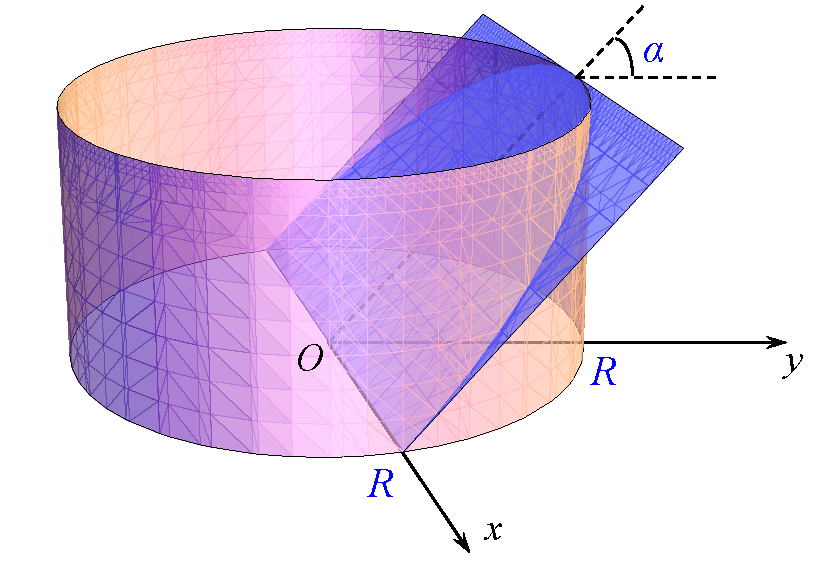
\includegraphics{./images/ch6/bucket.pdf}}
\end{center}

{\bf 例:}半径不等的两个木质球体,分别中间凿去一个以直径为轴的正圆柱体以及柱体下方的球冠,
剩下的环状部分高度均为$h$,问哪一个环状物体的体积更大。

[hint]:
$$V=\dint_{\sqrt{R^2-h^2}}^R2\pi x\sqrt{R^2-x^2}\d x=\df23\pi h^3$$
结果表明:剩余部分的体积与球半径无关!

{\bf 例:}试推导球的体积公式和球面上一块面积为$S$的球心锥的体积公式($rS/3$)

{\bf 例:}开口容器内的水在单位时间内的蒸发量与水的表面积成正比,证明:水的深度以常速率
下降且与容器形状无关。

[hint]:设水的表面积为$S$,则
$$\Delta V\approx S\Delta h\Rightarrow
\df{\Delta V}{\Delta t}\approx S\df{\Delta h}{\Delta t}$$
即
$$\df{\d V}{\d t}=S\df{\d h}{\d t}$$

\subsection{物理问题}

\subsubsection{平面物体的质心}
$y=f(x)(a<x<b)$密度均匀,其质心的横坐标为
$$\bar{x}=\df{\dint_a^bxf(x)\d x}{\dint_a^bf(x)\d x}$$

{\bf 例:}求右半圆的质心坐标。

{\bf 例:}$f(x)\in C[a,b]$且单调递增,证明:
$$\dint_a^bxf(x)\d x\geq\df{a+b}2\dint_a^bf(x)\d x$$
[hint]:物理意义:递增函数的形成的曲边梯形质心位于右侧。

证1:由$f(x)$单增,
$$\left(x-\df{a+b}2\right)\left(f(x\right)-f\left(
\df{a+b}2\right)\geq0$$
两边积分即得。

证2:记$c=\df{a+b}2$
\begin{align}
	\dint_a^b&(x-c)f(x)\d x\notag\\
	&=\left(\dint_a^c+\dint_c^b\right)(x-c)f(x)\d x\notag\\
	&=f(\xi_1)\dint_a^c(x-c)\d x+f(\xi_2)\dint_c^b(x-c)\d x\notag\\
	&=[f(\xi_1)-f(\xi_2)]\df{(b-a)^2}2\geq0
\end{align}

\subsubsection{变力沿直线做功}

{\bf 例:}一圆柱形的水桶高$5m$,底半径$3$m,桶内装满水,问要将桶内的水全部抽出,
需要做多少功(设重力加速度$g=10N/kg$)。

{\bf 例:}在由电量为$+q$的电荷产生的电场中,沿某一轴向将一个单位正电荷由距离
$a$移动到距离$b$的位置,问在该过程中,电场力共对该电荷做了多少功?

{\bf 电场力:}
$$F=k\df{q_1q_2}{r^2}$$

\subsubsection{水压}

{\bf 例:}某个圆柱形油桶底半径为$R$,所装油密度为$\rho$,
现将其装满油后横放,求其端面承受的压力。

\subsubsection{万有引力}

{\bf 例:}设有一长度为$l$,线密度为$\mu$的均匀细直棒,在其中垂线上距离棒$a$
处有一质量为$m$的质点$M$,求该棒对质点$M$的引力。

{\bf 计算结果:}
\begin{align}
	F&=-\dint_{-\frac l2}^{\frac l2}\df{Gam\mu}{(a^2+y^2)^{\frac32}}\d y
	=-\dint_{-\arctan\frac l{2a}}^{\arctan\frac l{2a}}\df{Gam\mu}{(a^2+(a\tan
	t)^2)^{\frac32}}\d (a\tan t)\notag\\
	&=-\df{Gm\mu}a\dint_{-\arctan\frac l{2a}}^{\arctan\frac
	l{2a}}\cos t\d t=-\df{Gm\mu}a\left.\sin t\right|_{-\arctan\frac
	l{2a}}^{\arctan\frac l{2a}}\notag\\
	&=-\df{2Gm\mu}a\sin\left(\arctan\df l{2a}\right)\notag
\end{align}
注意到$\sin x=\df{\tan x}{\sec x}=\df{\tan x}{\sqrt{1+\tan^2 x}}$,故
$$\sin\left(\arctan\df l{2a}\right)=\df{\frac{l}{2a}}
{\sqrt{1+\left(\frac{l}{2a}\right)^2}}=\df{l}{\sqrt{4a^2+l^2}}$$
代回前式即得$F=-\df{2Gm\mu l}{a\sqrt{4a^2+l^2}}$。

\section{反常积分}

{\bf 定积分存在的条件:}

$${I=\dint_a^bf(x)\d x}$$

\begin{enumerate} [(1)]
  \setlength{\itemindent}{1cm}
  \item {\bf 有限区间:}$a,b\ne \infty$
  \item {\bf 分段连续:}$f(x)$最多有限多个第一类间断点 
  \item {\bf 必要条件:}$f(x)$有界
\end{enumerate}

\subsection{无穷限的反常积分}

{\bf 定义6.5.1:}
$${\dint_a^{+\infty}f(x)\d x}
=\lim\limits_{t\to+\infty}\dint_a^tf(x)\d x$$
类似地,可以定义${\dint_{-\infty}^af(x)\d x}$和
${\dint_{-\infty}^{+\infty}f(x)\d x}$

Newton-Leibnitz公式 
  $$\dint_a^{+\infty}f(x)\d x=F(x)|_{a}^{+\infty}
  =\limx{+\infty}F(x)-F(a)$$
  
{\bf P381-例1:}计算以下无穷积分
$$\dint_{-\infty}^{+\infty}\df{1}{1+x^2}\d x$$

\begin{center}
	\resizebox{!}{5cm}{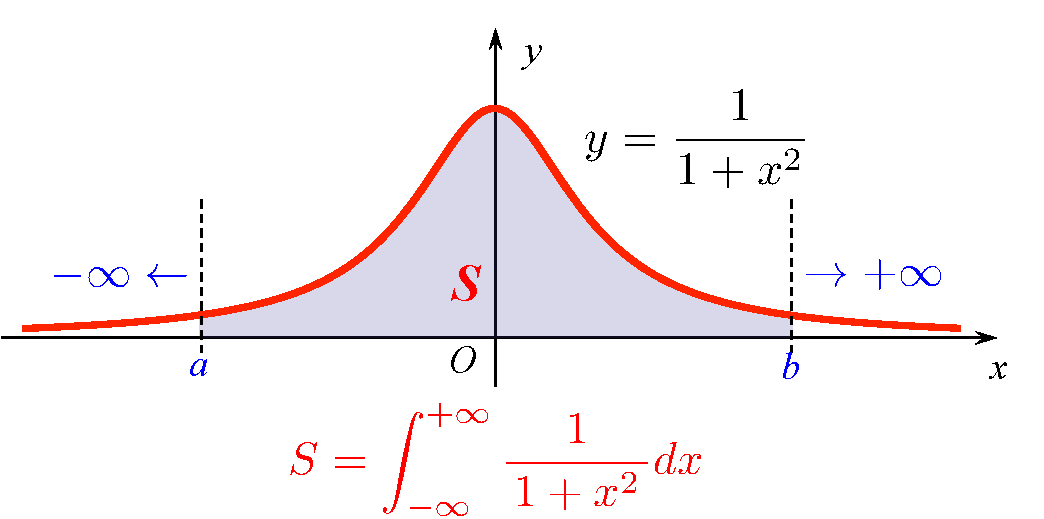
\includegraphics{./images/ch6/infint.pdf}}
\end{center}

{\bf P382-例3,P384-例5:}
\begin{enumerate}[(1)]
  \setlength{\itemindent}{1cm}
  \item 讨论$\dint_a^{+\infty}\df{\d x}{x^p},\;a>0, p>0$的敛散性; 
  \item 证明$$\dint_1^{n+1}\df 1{x^p}\d x<\sum\limits_{k=1}^n\df 1{k^p}
  <1+\dint_1^n\df{1}{x^p}\d x$$ 
  \item 根据以上结论给出$p$级数的判敛条件。
\end{enumerate}

\begin{shaded}
	{\bf Gabriel's Horn Paradox}(加百利喇叭的悖论)
	
	Gabriel是圣经故事中的天使,他吹奏一支长喇叭让魔鬼坠入地狱。关于长喇叭有如下的一个悖论
	(据说由Torricelli(托里拆利)提出):设Gabriel喇叭由区县$y=\df1x(x\geq 1)$
	围绕$x$轴旋转而成,证明:
	\begin{enumerate} [(1)]
  	  \setlength{\itemindent}{1cm}
	  \item 喇叭的体积是一个有限值
	  \item 喇叭的表面积为无穷大
	  \item 有前面的结论应该可以推论出这样的结果:Gabriel喇叭的内部可以被有限数量
	  的油漆填满,但同时,任何有限数量的漆都无法刷遍其内表面!该如何解释这个悖论呢?
	\end{enumerate}
	[hint]:
	(1)体积为
	$$V=\dint_1^{+\infty}\pi\left(\df1x\right)^2\d x=\pi$$
	(2)表面积
	$$A=\dint_1^{+\infty}2\pi y\d s=2\pi\dint_1^{+\infty}
	\df{\sqrt{x^4+1}\d x}{x^3}>\dint_1^{+\infty}\df1x\d x=+\infty$$
	(3)如果涂在表面上的漆的厚度可以是任意小,则任意有限数量的漆都可以刷遍整个喇叭。
	
	一个类似的假定:对于平面区域$D:x\geq0,y\in[0,1]$,给定一个单位质量的金箔,
	只要我们允许金珀铺的任意薄(厚度$h(x)=e^{-x}$),则可以将整个区域$D$铺满。
\end{shaded}

\subsection{无界函数的反常积分}

{\bf 定义6.5.2:}
\begin{enumerate} [(1)]
  \setlength{\itemindent}{1cm}
  \item {\it 瑕点:}无穷间断点 
  \item 设$a$为$f(x)$的瑕点,{\it 瑕积分:}
  $$\dint_a^bf(x)\d x=\limx{a^+}\dint_t^bf(x)\d x$$
\end{enumerate}

{\bf P386-例6:}计算
$$\dint_0^a\df{1}{\sqrt{a^2-x^2}}\d x,\;a>0$$

{\bf P387-例7:}讨论瑕积分的收敛性
\begin{enumerate}[(1)]
  \setlength{\itemindent}{1cm}
  \item $\dint_{-1}^1\df{\d x}{x^2}$ 
  \item $\dint_{-1}^1\df{\d x}{x}$
\end{enumerate}

{\bf 例:}计算
$$\dint_0^{+\infty}\df{\d x}{\sqrt{x(x+1)^3}}$$

\subsection{反常积分收敛性的判定}

{\bf 定理6.5.3:}(比较判别法)
设$f(x),g(x)$在$[a,+\infty)$上连续,且
$$0\leq f(x)\leq g(x),\quad x\in[a,+\infty)$$ 
\begin{enumerate}[(1)]
  \setlength{\itemindent}{1cm}
  \item
  $\dint_a^{+\infty}g(x)\d x$收敛$\Rightarrow\dint_a^{+\infty}f(x)\d x$收敛 
  \item $\dint_a^{+\infty}f(x)\d x$发散$\Rightarrow\dint_a^{+\infty}g(x)\d x$发散
\end{enumerate}

{\bf P388-例1:}讨论以下无穷积分的敛散性
\begin{enumerate}[(1)]
  \setlength{\itemindent}{1cm}
  \item $\dint_2^{+\infty}\df{1+\sin x}{x^2}\d x$ 
  \item $\dint_1^{+\infty}\df{\d x}{\sqrt[3]{x^4+1}}$
\end{enumerate}

{\bf 定理}(极限判别法)
设$f(x),g(x)$在$[a,+\infty)$上连续,$0\leq f(x)\leq g(x)$,且
$$\limx{+\infty}\df{f(x)}{g(x)}=l$$ 
\begin{enumerate}[(1)]
  \setlength{\itemindent}{1cm}
  \item $0<l<+\infty$,两个无穷积分同敛散 
  \item
  $l=0$,$\dint_a^{+\infty}g(x)\d x$收敛
  $\Rightarrow\dint_a^{+\infty}f(x)\d x$收敛 
  \item
  $l=+\infty$,$\dint_a^{+\infty}f(x)\d x$发散
  $\Rightarrow\dint_a^{+\infty}g(x)\d x$发散
\end{enumerate}

{\bf 例:}判定以下反常积分的收敛性
\begin{enumerate}[(1)]
  \setlength{\itemindent}{1cm}
  \item $\dint_1^{+\infty}\df{\d x}{x\sqrt{1+x^2}}$ 
  \item $\dint_1^{+\infty}\df{x^{3/2}}{1+x^2}\d x$ 
  \item $\dint_1^{+\infty}\df{\arctan x}{x}\d x$
\end{enumerate}

{\bf 定理}(绝对收敛性)设$f(x)$在$[a,+\infty)$上连续,
若$\dint_a^{+\infty}|f(x)|\d x$收敛,则
$\dint_a^{+\infty}f(x)\d x$收敛。

{\bf 例:}讨论反常积分$\dint_0^{+\infty}e^{-ax}\sin bx\d x\;(a>0)$的敛散性。

{\bf 例:}判定下列积分的敛散性
\begin{enumerate}[(1)]
  \setlength{\itemindent}{1cm}
  \item $\dint_1^3\df{\d x}{\ln x}$ 
  \item $\dint_0^1\df{\d x}{\sqrt{(1-x^2)(1-k^2x^2)}}\;(k^2<1)$ 
  \item $\dint_0^1\df 1{\sqrt{x}}\sin\df 1x\d x$
\end{enumerate}

\subsection{$\Gamma$函数}

$${\Gamma(s)=\dint_0^{+\infty}e^{-x}x^{s-1}\d x\;(s>0)}$$

\begin{enumerate}[(1)]
  \setlength{\itemindent}{1cm}
  \item $\Gamma(s+1)=s\Gamma(s)$ 
  \item $\lim\limits_{s\to 0+}\Gamma(s)= +\infty$ 
  \item $\Gamma(s)\Gamma(1-s)=\df{\pi}{\sin \pi s}\;(0<s<1)$ 
  \item $2\dint_0^{+\infty}e^{-x^2}\d x=\Gamma\left(\df 12\right)=\sqrt{\pi}$
\end{enumerate}


\newpage

\section*{习题与课后思考题}

\section*{课后作业}

\begin{itemize}
  \item 习题6.1:3(1,3),4,5(4,5,6),6
  \item 习题6.2:1(5-8),2,3(3,4),4,6,7,8,13,15
  \item 习题6.3:4-6
  \item 习题6.4:2,5,6(1),8,10,11,15,16,19
  \item 习题6.5:1(4-6),2(1,4,6),5,8
\end{itemize}

{\bf 【课堂练习与思考题】}

\begin{itemize}
  \item 习题6.1:7,8,9,10
  \item 习题6.3:8,9,12,14,18
  \item 习题6.4:1-30其余各题
\end{itemize}

{\bf 例:}$a>0,c\in(0,e^a)$,证明:
$$\dint_0^a|e^x-c|\dx\geq(e^{\frac a2}-1)^2$$

\newpage

\section[不定积分计算的一些典型方法]{不定积分计算的一些典型方法}

{\bf 例:}计算不定积分
\begin{enumerate}[(1)]
  \setlength{\itemindent}{1cm}
  \item $\dint\df1{x^4(1+x^2)}\d x$
  \item $\dint(\tan x+\cot x)^2\d x$
  \item $\dint\df1{1+\sin x}\d x$
  \item $\dint\df1{\sin2x+2\sin x}\d x$
\end{enumerate}

% [hint]:
% (1) 方法1:
% $$\mbox{原式}=\dint\df{(1+x^2)-x^2}{x^4(1+x^2)}\d x
% =-\df1{3x^3}+\df1x+\arctan x+C$$
% 
% 方法2:
% $$\mbox{原式}=\dint\df{(1-x^4)+x^4}{x^4(1+x^2)}\d x$$
% 
% (2)
% $$\tan x-\cot x+C$$
% 
% (3)方法1:
% $$\mbox{原式}=\dint\df1{1+\cos\left(x-\df{\pi}2\right)}\d x=\ldots
% =\tan\df{2x-\pi}4+C$$
% 
% 方法2:
% $$\mbox{原式}=\dint\df{1-\sin x}{\cos^2x}\d x=\ldots=\tan x-\sec x+C$$
% 
% (4)方法1:
% $$\mbox{原式}=\df14\dint1{\sin\df x2\cos x2\cos^2\df x2}\d\df x2
% =\df14\dint\df{1+\tan^2\df x2}{\tan\df x2}\d\tan\df x2
% =\df14\ln\left|\tan\df x2\right|+\df18\tan^2\df x2+C$$
% 
% 方法2:
% $$\mbox{原式}=\dint\df{1-\cos x}{2\sin^3x}\d x=\ldots
% =\df14\ln|\csc x-\cot x|-\df14\csc x\cot x+\df14\csc^2x+C$$

\begin{shaded}

{\bf 提示:}通过代数恒等变换、三角恒等变换等方法,把所求的积分化为基本积分公式中
的积分或其他易于积分的形式。为此,需要熟练掌握基本的积分公式,这样才能有针对性地对
被积函数进行恒等变形。

\end{shaded}

{\bf 例:}计算不定积分
\begin{enumerate}[(1)]
  \setlength{\itemindent}{1cm}
  \item $\dint\df{2x+3}{\sqrt{1+2x-x^2}}\d x$
  \item $\dint\df1{1+e^x}\d x$
  \item $\dint\df1{x(x^n+a)}\d x,\;(a\ne 0,n\in\mathbb{Z}_+)$
  \item $\dint\df{x^2+1}{x^4+1}\d x$
\end{enumerate}

% [hint]:
% (1)方法1:
% $$\mbox{原式}=\dint\df{5-(2-2x)}{\sqrt{1+2x-x^2}}\d x
% =5\dint\df{\d(x-1)}{\sqrt{2-(x-1)^2}}-\dint\df{\d(1+2x-x^2)}
% {\sqrt{1+2x-x^2}}$$
% $$=5\arcsin\df{x-1}{\sqrt 2}-2\sqrt{1+2x-x^2}+C$$
% 
% 方法2:令$x-1=\sqrt 2\sin t$
% 
% (2)方法1:
% $$\mbox{原式}=\dint\df{1+e^x-e^x}{1+e^x}\d x=x-\ln(1+e^x)+C$$
% 
% 方法2:
% $$\mbox{原式}=\dint\df{e^x}{e^x(1+e^x)}\d x$$
% 
% 方法3:
% $$\mbox{原式}=\dint\df{e^{-x}}{1+e^{-x}}\d x$$
% 
% (3)方法1:
% $$\mbox{原式}=\dint\df{x^{n-1}}{x^n(x^n+a)}\d x
% =\ldots=\df1{na}\ln\left|\df{x^n}{x^n+a}\right|+C$$
% 
% 方法2:
% $$\mbox{原式}=\df1a\dint\df{a+x^n-x^n}{x(x^n+a)}\d x$$
% 
% (4)
% $$\mbox{原式}=\dint\df{1+\df1{x^2}}{x^2+\df1{x^2}}\d x
% =\df1{\sqrt2}\arctan\df{x^2-1}{\sqrt2x}+C$$

\begin{shaded}

{\bf 提示:}对于不易观察出微分形式的不定积分,有时需要进行适当的恒等变形,
凑成$\dint f(\phi(x))\phi'(x)\d x=\dint f(\phi(x))\d\phi(x)$
的形式,利用凑微分法求出不定积分。

\end{shaded}

{\bf 例:}计算不定积分
\begin{enumerate}[(1)]
  \setlength{\itemindent}{1cm}
  \item $\dint\cos3x\cos2x\d x$
  \item $\dint\sin^4x\cos^2x\d x$
  \item $\dint\sin^3x\cos^3x\d x$
  \item $\dint\tan^3x\sec^4x\d x$
  \item $\dint\tan^3x\cos x\d x$
  \item $\dint\cot^3x\csc^5x\d x$
\end{enumerate}


\begin{shaded}
{\bf 提示:}对积分

1)\;$\dint\sin ax\cos bx\d x$\;2)$\dint\sin ax\sin bx\d x$\;
3)$\dint\cos ax\cos bx\d x$

4)$\dint\sin^mx\cos^nx \d x$\;5)$\dint\tan^mx\sec^nx\d x$\;
6)$\dint\cot^mx\csc^nx\d x$

主要通过三角变换来凑积分求解。
\begin{enumerate}[(1)]
  \item 1)-3),和差化积;
  \item 4),当$n$或$m$为奇数时,分离出一个$\cos x$(或$\sin x$),凑出
  $\d\sin x$(或$\d\cos x$),在利用$\sin^2x+\cos^2x=1$将剩余部分都化为
  $\cos x$或$\sin x$的多项式;若$m$和$n$均为偶数,利用倍角公式将函数降阶
  再积分即可;
  \item 5),$m$为奇数时,分离出$\sec x\tan x$,可凑出$\d\sec x$,再将
  剩余部分都化为关于$\sec x$的多项式;当$n$为偶数时,分离出$\sec^2x$,可凑出
  $\d\tan x$,将剩余部分化为$\tan x$的多项式积分;
  \item 6)可参考5)的思路。
\end{enumerate}
\end{shaded}

{\bf 例:}计算不定积分
\begin{enumerate}[(1)]
  \setlength{\itemindent}{1cm}
  \item $\dint\ds\df2{x+\sqrt{1-x^2}}\d x$
  \item $\dint\ds\df1{x\sqrt{x^2-1}}\d x$
  \item $\dint\ds\df{\sqrt{1+x^2}}{x^2}\d x$
  \item $\dint\ds\df1{\sqrt{(9x^2-6x-1)^3}}\d x$
  \item $\dint\ds\df{1-x}{\sqrt{x(4-x)}}\d x$
\end{enumerate}
% 
% [hint]:
% (1)$x=\sin t$,
% $$\mbox{原式}=\arcsin x+\ln\left|x+\sqrt{1-x^2}\right|+C$$
% 
% (2)方法1:$x=\sec t$
% $$\mbox{原式}=\arccos\df1x+C$$
% 
% 方法2:$x>1$时,令$x=\df1t$;$x<-1$时,令$x=-\df1t$
% 
% 方法3:$t=\sqrt{x^2-1}$,
% $$\mbox{原式}=\arctan\sqrt{x^2-1}+C$$
% 
% 方法4:
% $$\mbox{原式}=\dint\df{1}{x^2}\d\sqrt{x^2-1}
% =\dint\df1{1+(\sqrt{x^2-1})^2}\d\sqrt{x^2-1}$$
% 
% (3)$x=\tan t$
% $$\mbox{原式}=\ln\left|x+\sqrt{1+x^2}\right|
% -\df{\sqrt{1+x^2}}{x}+C$$
% 
% (4)$x=\df{\sqrt2}3\sec t+\df13$
% $$\mbox{原式}=-\df16\df{3x-1}{\sqrt{9x^2-6x-1}}+C$$
% 
% (5)方法1:
% $$\mbox{原式}=\df12\dint\df{4-2x-2}{\sqrt{x(4-x)}}\d x
% =\dint\df{\d [x(4-x)]}{2\sqrt{x(4-x)}}-\dint\df{\d x}{\sqrt{x(4-x)}}
% =\sqrt{x(4-x)}-2\arcsin\df{\sqrt x}2+C$$
% $$\dint\df{\d x}{\sqrt{x(4-x)}}=\dint\df{\d x}{\sqrt{4-(x-2)^2}}
% =\arcsin\df{x-2}2+C$$

\begin{shaded}
{\bf 提示:}被积函数含根式形式如$\sqrt{a^2\pm x^2}$,$\sqrt{x^2-a^2}$等,
常采用三角代换、倒代换等,但不要只拘泥于这种代换,应具体问题具体分析,如(5)用凑微分
法更好。

被积函数含$\sqrt{x^2-a^2}$型时,令$x=a\sec t$或者$x=a\csc t$,视$0<t<\df{\pi}2$。
\end{shaded}

{\bf 例:}计算不定积分
\begin{enumerate}[(1)]
  \setlength{\itemindent}{1cm}
  \item $\dint\df{e^x(1+e^x)}{\sqrt{1-e^{2x}}}\d x$
  \item $\dint\df{\ln x}{x\sqrt{1+\ln x}}\d x$
\end{enumerate}

% [hint]:(1)方法1:$e^x=\sin t$,
% $$\mbox{原式}=\arcsin e^x-\sqrt{1-e^{2x}}+C$$
% 
% 方法2:$\sqrt{1-e^{2x}}=t$
% 
% $$\mbox{原式}=\arccos\sqrt{1-e^{2x}}-\sqrt{1-e^{2x}}+C$$
% 
% 方法3:
% $$\mbox{原式}=\dint\df{e^x\d x}{\sqrt{1-e^{2x}}}
% +\dint\df{e^{2x}\d x}{\sqrt{1-e^{2x}}}$$
% 
% (2)方法1:
% $$\mbox{原式}=\dint\df{1+\ln x-1}{\sqrt{1+\ln x}}\d(\ln x)
% =\df23(1+\ln x)^{\frac32}-2\sqrt{1+\ln x}+C$$
% 
% 方法2:$\sqrt{1+\ln x}=t$

\begin{shaded}
{\bf 提示:}果断进行代换,将不易处理的部分代换成一个变量。
\end{shaded}

{\bf 例:}计算不定积分
\begin{enumerate}[(1)]
  \setlength{\itemindent}{1cm}
  \item $\dint x^3e^{-x^2}\d x$
  \item $\dint (x+1)\sin^2x\d x$
  \item $\dint x\ln(1+x^2)\d x$
  \item $\dint\arctan\sqrt x\d x$
  \item $\dint\ln\left(1+x+\sqrt{2x+x^2}\right)\d x$
  \item $\dint\df{\sin^2x}{e^x}\d x$
  \item $\dint e^{2x}(\tan x+1)^2\d x$
  \item $\dint\df{xe^x}{(1+x)^2}\d x$
  \item $\dint(1-2x^2)e^{-2x^2}\d x$
  \item $\dint\df{x+\sin x}{1+\cos x}\d x$
  \item $\dint\df{1+\sin x}{1+\cos x}e^x\d x$
  \item $\dint\df{e^{\arctan x}}{(1+x^2)^{3/2}}$
  \item $\dint\df{\ln x\d x}{(1+x^2)^{3/2}}$
\end{enumerate}

\begin{shaded}
{\bf 提示:}被积函数为幂函数(或多项式函数)与指数函数、三角函数、对数函数或反三角函数
乘积的积分,可考虑分布积分法。
\end{shaded}

{\bf 例:}计算不定积分
\begin{enumerate}[(1)]
  \setlength{\itemindent}{1cm}
  \item $\dint\df{x^5}{1+x^3}\d x$
  \item $\dint\df1{1+x^4}\d x$
  \item $\dint\df{1-x^7}{x(1+x^7)}\d x$
  \item $\dint\df{x^{11}\d x}{x^8-4x^4+3}$
\end{enumerate}

\begin{shaded}
{\bf 提示:}有理函数积分。
\end{shaded}

{\bf 例:}计算不定积分
\begin{enumerate}[(1)]
  \setlength{\itemindent}{1cm}
  \item $\dint\df{\cos x\d x}{1+\cos x}$
  \item $\dint\df1{2+\sin x}\d x$
  \item $\dint\df1{\sin x+\cos x}\d x$
  \item $\dint\df{\sin x\d x}{\sin x+\cos x}$
  \item $\dint\df{\sin2x\d x}{\sin^2x+\cos x}$
  \item $\dint\df{\cos^2x\d x}{1+\cos^2x}$
\end{enumerate}

\begin{shaded}
{\bf 提示:}三角函数的有理式积分,总可以使用万能公式化为有理函数来计算。但其后的计算
往往相当复杂,因此,结合三角函数的其他变化公式,进行适当变形寻求积分的途径,往往更加
简单些。
\end{shaded}

{\bf 例:}计算不定积分
\begin{enumerate}[(1)]
  \setlength{\itemindent}{1cm}
  \item $\dint\df{\sqrt[3]x}{x(\sqrt x-\sqrt[3]x)\d x}$
  \item $\dint\df{\d x}{x\sqrt{1+\sqrt{x^3}}}$
  \item $\dint\sqrt{\df{x+1}{x-1}}\d x$
  \item $\dint\df{\d x}{\sqrt(x-1)^3(x-2)}$
  \item $\dint\df{xe^x\d x}{\sqrt{e^x+1}}$
\end{enumerate}

% [hint]:(3)$\sqrt{\df{x+1}{x-1}}=t$或直接分子有理化后凑微分
% 
% (4)$\sqrt{\df{x-2}{x-1}}=t$
% 
% (5)$\sqrt{e^x+1}=t$

\begin{shaded}
{\bf 提示:}含有$\ds\sqrt[n]{\df{ax+b}{cx+d}}$的无理函数积分,理论上用根式代换
可以求出其积分。但化为有理函数积分后,往往计算量较大,应优先考虑通过恒等变形凑微分来计算。
\end{shaded}